Stružnica je najstarejši obdelovalni stroj,
ki se ga uporablja pri struženju. Še vednon se
veliko uporabljajo v strojništvu in lesarstvu,
tako da skoraj ni delavnice brez tega obdelovalnega stroja.
Za razliko od rezkalnih strojev, glavno krožno gibanje opravlja
obdelovanec, zato se največkrat na stružnici obdelujejo rotacijsko
simetrični kosi. Obdelujejo se lahko tudi rotacijsko nesimetrični kosi,
vendar za njih potrebujemo posebno vpetje, obdelana površina pa je
vedno vzporedna z osjo rotacije.

\noindent Glavni deli standardne stružnice so:
\begin{itemize}
	\item Postelja
	\item Vretenjak
	\item Podajalni menjalnik
	\item Sani s suporti
	\item Konjiček
	\item Lineta
\end{itemize}

In so prikazani na spodnji sliki \ref{img:deli_struznice} univerzalne klasične stružnice.
\begin{figure}[H]
	\begin{center}
		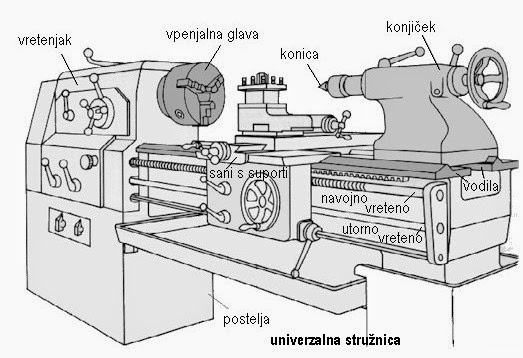
\includegraphics[width=10cm]{deli_struznice.jpg}
		\caption{Glavni deli stružnice
			\cite{deli_struznice}}
		\label{img:deli_struznice}
	\end{center}
\end{figure}

\noindent Glede na glavne dele in njihovo orientacijo in namestitev razlikujemo
predvsem naslednje vrste stružnic:
\begin{itemize}
	\item Univerzalna stružnica
	\item Čelna stružnica
	\item Karoselna stružnica
	\item Revolverska stružnica
\end{itemize}

\noindent Iz navedenih oblik pa so se razvile še posebej specializirane
stružnice kot naprimer:
\begin{itemize}
	\item Kopirna ali podstružilna stružnica
	\item Avtomatska stružnica
	\item Numerično krmiljena stružnica (ali krajše CNC stružnica)
\end{itemize}